\documentclass[letterpaper,twocolumn,10pt]{article}
\usepackage{usenix2019_v3}

% to be able to draw some self-contained figs
\usepackage{tikz}
\usepackage{amsmath}
\usepackage{amsfonts}
% inlined bib file
\usepackage{filecontents}
\usepackage{listings}
\usepackage{color}
\usepackage{longtable}
\usepackage{mathptmx}
\usepackage{setspace}
% for author-year citation style
% \usepackage{natbib}
\usepackage{lscape}
\usepackage{graphicx}
\usepackage{scalerel}
\usepackage[export]{adjustbox}
\usepackage{siunitx}
\usepackage{subfig}
\usepackage{caption}
\usepackage{multirow}

\usepackage{fullpage}
\usepackage{times}
\usepackage{fancyhdr,graphicx,amsmath,amssymb}
\usepackage[ruled,vlined]{algorithm2e}
\include{pythonlisting}

\definecolor{dkgreen}{rgb}{0,0.6,0}
\definecolor{gray}{rgb}{0.5,0.5,0.5}
\definecolor{mauve}{rgb}{0.58,0,0.82}

\lstset{frame=tb,
  language=Java,
  aboveskip=3mm,
  belowskip=3mm,
  showstringspaces=false,
  columns=flexible,
  basicstyle={\small\ttfamily},
  numbers=none,
  numberstyle=\tiny\color{gray},
  keywordstyle=\color{blue},
  commentstyle=\color{dkgreen},
  stringstyle=\color{mauve},
  breaklines=true,
  breakatwhitespace=true,
  tabsize=3
}
\graphicspath{{proj_graphs/}}
\begin{document}
%-------------------------------------------------------------------------------

%don't want date printed
\date{}

% make title bold and 14 pt font (Latex default is non-bold, 16 pt)
\title{\Large \bf Optimizing LeCar and Convolutional Neural Network Approaches for Cache Replacement Policy}

%for single author (just remove % characters)
\author{
{\rm Yilin Han}\\
yilinhan10@cs.toronto.edu\\
University of Toronto
\and
{\rm Mengxuan Lyu}\\
shawnlyu@cs.toronto.edu\\
University of Toronto
% copy the following lines to add more authors
% \and
% {\rm Name}\\
%Name Institution
} % end author

\maketitle

%-------------------------------------------------------------------------------
\begin{abstract}
%-------------------------------------------------------------------------------
Improving system performance with caching replacement technique is always one of the hottest topics in systematic research. In this project, we proposed a new cache eviction algorithm, namely, LeCar\_Opt, which outperforms ARC when the cache size is small. Furthermore, machine learning models are used to learn the cache replacement patterns on real-world workload. We implemented, tuned and analyzed the Multilayer Perceptron, Convolutional Neural Network, and Decision Tree on the OPT solutions. It is concluded that machine learning models are capable of learning OPT patterns with adequate hyperparameter tuning.


\end{abstract}


%-------------------------------------------------------------------------------
\section{Introduction}

Historically, the development of CPU is much faster than the improvement of disk bandwidth. Cache replacement algorithms as one of the oldest and fundamental computer problems play an essential role to resolve this gap. The performance of caching algorithms strongly influence the system performance. Especially in the past decade,  with the advance of the big data technology, more and more data are required to be stored and processed in the modern software systems. 

Cache is used to balance the performance difference between high-speed devices and low-speed ones. For example, the data in the memory is written to the Hard Disk Drive (HDD). Since HDD is much slower than the memory, it takes a long time to complete a task in theory, which results in very slow writing performance. In order to resolve the speed difference between memory and HDD, a buffer is created between them to temporarily store the data. 

The performance of a cache algorithm is measured by the hit rate. If the hit ratio is low, it means the cache is used inefficiently. Moreover, it may affect the speed of the entire system. In this project, multiple classic and ML-based caching algorithms were investigated. The results were further compared and analyzed with the traditionally caching replacement algorithms.

\section{Background}

\subsection{Existing Cache replacement policies}
Traditional caching replacement algorithms mainly utilize the frequency of a page request or the recency of a page request time as a standard to identify which page in the cache needs to be evicted in a replacement operation. The operation in these cache algorithms is relatively simple, and basically, their performance is strongly influenced by the incoming data: they may only perform well on one type of incoming data pattern, and the hit ratio gets significantly reduced on other data requesting patterns. There are two main types of traditional cache algorithms: LRU and LFU.

Least Recently Used (LRU) cache replacement algorithm is the most widely used caching algorithm in the industry. As the name states, The key idea of LRU is performing cache replacement with the least recently used page\cite{mattson1970evaluation}. The implementation is simple as well. It usually uses a deque\cite{WinNT} and put the most recent page in the tail of the queue. The page is appended to the tail upon a hit on the cache. While replacing a page, it evicts the head page on the queue. This implementation is extremely cheap and the performance is outstanding. In real applications, most of the systems use LRU as their main method. The algorithm shows the superiority to the locality of reference exhibited in the request sequence. However, It is vulnerable to sequential disk scan, such as when the sequential requested data size is larger than the cache size, LRU has no effect in the cache. 

Least Frequently Used (LFU) cache replacement algorithm tends to evict the least frequently used page in the cache. This is based on the assumption that the pages with higher request count are more likely to be requested to be referenced again in the near future\cite{coffman1973operating}. In terms of the implementation, this requires extra overhead to maintain the page number and corresponding frequency counts. Hashmap is normally the best to keep track of the pages. However, the cost to keep the hashmap in the memory could be extremely high when the system is running for a long time. LFU also has disadvantages. It adapts poorly to variate access patterns by accumulating stale pages with past high-frequency counts. For example, some pages are referenced a large number of times at beginning but not used them in the future, these pages would stay in the memory for a long time. 

The Adaptive Replacement Cache (ARC) algorithms combine the LRU and LFU algorithms\cite{megiddo2003arc}. ARC proposed a novel approach that not only cares about the recency and frequency but also includes the history of evicted pages into considerations\cite{consuegra2015analyzing}. It divides the cache into two LRU lists: T1 and T2. T1 is maintained to cover the short-term utility such that a new page is always stored in the T1 list when it first time entered the cache. The pages in T1 will gradually move to T2 when they are accessed more than once. This means T2 list represents the frequency feature of the page just as LFU. Thus, the long-term utility is preserved in T2. In addition to using T1 and T2 list to represent the cache, ARC also maintains a history list with the same size as cache. They are being called “Ghost” list B1 and B2 were corresponding to T1 and T2 respectively. B1 stores the pages, which is not currently in the cache, that have been recently deleted from T1, and B2 stores the pages recently deleted from T2. B1 and B2 are also acting in LRU manner. The unique characteristic of ARC is the ability of self-tuning. The size of T1 may grow or shrink relative to T2 when there is a hit in B1 or B2. This adaptive feature makes the algorithm capable of adjusting the T1 and T2 size in order to overcome the above-mentioned disadvantages from LRU and LFU.

Belady's Optimal Replacement Policy (OPT) is considered as the best cache replacement algorithm in this field\cite{belady1966study}\cite{mattson1970evaluation}. OPT traces the future blocks that will be brought to cache in order to pick the best candidate to evict. It is not implementable because no one could truly predict the future requests in practice. Nevertheless, it is still used as the performance benchmark for cache algorithms testing. 


\subsection{Machine learning based approaches}

Increasing attention is cast on Machine Learning (ML) in recent years, which is a field where algorithms are applied on computers to learn from previous data for predicting similar patterns in new data, without explicitly programmed. It can be generally categorized into three main approaches: supervised learning, unsupervised learning, and reinforcement learning\cite{article}. 

Researchers have shown that ML could be applied to improve cache replacement policies: \cite{im2018snn} proposed an ML-based caching system to notably decrease the load of content servers by improving caching decisions; \cite{ari2002acme} developed the ACME system which utilizes ML to learn from multiple cache replacement strategies before making the recommendation about which to evict; \cite{article} showed that supervised learning algorithms like Support Vector Machines and Naive Bayes would lead to considering improving on hit ratio when combined with traditional algorithms like LRU, LFU. Besides, with the increasing computational powers, Neural Networks like MLP and CNN furthermore enhance the learning ability of machines.

As revealing internal relations and capturing hidden patterns among page requests would remarkably improve the efficiencies of cache replacement policies, ML-based approaches showed promising applications in this field. In this work, decision trees \cite{brodley1995multivariate}, MLP, and CNN\cite{schmidhuber2015deep} would be implemented to make decisions over page evictions when there is a cache miss happening.

\section{Methodology}

\subsection{Dataset}

The FIU\cite{koller2010deduplication} computer science department workload is utilized as the training and testing dataset. The data was collected for three weeks and consist of all I/O traces on two web-servers, one email server, and one file server. Our experiments were conducted on email server data, since it is the most heavily used system in the data set. Each mail data file is roughly 1.8 gigabytes in size. FIU workload trace was generated by blktrace\cite{brunelle2007blktrace} command. Each record from the workload file is corresponding to the nine features of a block request: time-stamp, process id, process name, logical block address, request size, operation type, major device number, minor device number, and block hash. In our experiment, only the integer-typed logical block address is used.

\subsection{Implementations}

\subsubsection{LeCar - Opt}

LeCar\cite{vietri2018driving} is a framework that self-proclaims as an Reinforcement Learning (RL) based cache algorithm. It agrees to the fact that a single cache replacement strategy could not satisfy the daily workload scenarios. Both LRU and LFU have drawbacks as described above. With such an assumption, LeCar leverages the reinforcement learning concept, called regret minimization, to switch policies between LRU and LFU. It maintains two weight factors for choosing LRU or LFU policies perspectively and two history list corresponding to the evicted pages after conducting LRU policy or LFU policy. For example. If there is a hit from LRU evicted pages, the weight of using LFU will be increased, and vice versa. With adjusted weights, a random number is generated to select the next policy. 

In the early phase of the project, the LeCar algorithm was reproduced, but soon two unacceptable problems were noticed. First, it is not an RL-based algorithm even though they claimed so. LeCar does not have any well-known features that an RL or ML algorithm has and they falsely impose the reinforcement learning concept or terms on the wrong field. For example, reinforcement learning results in a decision matrix during the training and learning process, then the algorithm uses the decision matrix alone in the later testing. However, LeCar is an online algorithm, which makes policy change decision after each weight adjustment. The next policy to be used in purely random and this does not involve any learning or training. The second problem of Lecar is overfitting. The LeCar converges easily on FIU workload with small learning rate and discount rate, thus tuning the algorithm is impossible. 

Even through LeCar is problematic, we proposed LeCar\_Opt (Algorithm 1) based on the two ideas borrowed from LeCar. First, handling the workload of only two fundamental policies, LRU and LFU. The choice of choosing either policy is dependent on the current environment. In addition, the history of LRU and LFU evicted pages are being tracked. 

In Algorithm 1, the LeCar\_OPT manages a First In First Out (FIFO)lists of history evicted pages for LRU and LFU perspectively. The size of the list is equivalent to the cache size. The intent is that the algorithm is detecting the patterns from the history list. Specifically, the policy is switched when there is the following cases happens: 


- Case 1: If the current policy is LRU and there is a hit on the evicted page history for LRU, besides, if the requested page has the highest frequency among all the pages frequencies in the cache, then the policy is switched to LFU. This is aiming to go against sequential disk read patterns. With LFU, the high-frequency pages will be stored in the cache. 


- Case 2: There is also a condition that setup to switch LFU to LRU: if the current policy is LFU, and the hit on the LFU evicted page history list could potentially be a cache hit if the policy was LRU. This is completed by using a counter to record the number of page replacement after the last policy switch. The design is for detecting the recency pattern.

The policy switching is not only decided by whether there is a hit on the corresponding history list but also decided by its recency and frequency as described in the above two cases. At the early stage while developing the algorithm, the hit ratio reduced due to frequent switching of the policy. That is because some pages have stayed in the history pages for too long, causing a false signal to change the policy. For example, the page can stay in LFU evicted page history for a long period of time, that exceed the size. The page is considered invalid because the page is not going to generate a hit even the algorithm uses LRU. 

\begin{algorithm}
\SetAlgoLined
\KwIn{requested page $q$}
    initialization\;
    \eIf{$q$ is in $cache$}{
            UPDATE\_RECENCY($q$)\;
            UPDATE\_FREQUENCY($q$)\;
        }
    {
        \uIf{$q$ is in $lru\_evicted\_history$ AND $current\_policy$ is $lru$}{
            $max\_frequency$ $\leftarrow$ MAX(GET\_FREQUENCY($cache$))\;
            \uIf{FREQUENCY($q$) $\textgreater$ $max\_frequency$}{
                $lru\_evicted\_history$.DELETE$(q)$\;
            }
        }
        \ElseIf{$q$ is in $lfu\_evicted\_history$ AND $current\_policy$ is $lfu$}{
            \If{$evicted\_page\_count$ $\geq$ $cache.size$ }{
                $lfu\_evicted\_history$.DELETE$(q)$)\;
            }
        }
        \bigbreak
        \uIf{$q$ is in $lru\_evicted\_history$ AND $current\_policy$ is $lru$}{
             $lru\_evicted\_history$.DELETE$(q)$\;
             $current\_policy$ $\leftarrow$ $lfu$\;
        }
        \ElseIf{$q$ is in $lfu\_evicted\_history$ AND $current\_policy$ is $lfu$}{
            $cache$ $\leftarrow$ SORT(GET\_RECENCY($cache$))\;
            $lfu\_evicted\_history$.DELETE$(q)$\;
            $current\_policy$ $\leftarrow$ $lru$\;
        }
        \bigbreak
        \If{$cache$ is FULL}{
            \uIf{$current\_policy$ is $lru$}{
                $victim$ $\leftarrow$ GET\_LEAST\_RECENCY($cache$)\;
                \If{$lru\_evicted\_history$ is FULL}{
                    $lru\_evicted\_history$.DELETE\_HEAD()\;
                }
                $lru\_evicted\_history$.APPEND($victim$)\;
            }
            \ElseIf{$current\_policy$ is $lfu$}{
                $victim$ $\leftarrow$ GET\_LEAST\_FREQUENCY($cache$)\;
                \If{$lfu\_evicted\_history$ is FULL}{
                    $lfu\_evicted\_history$.DELETE\_HEAD()\;
                }
                $lfu\_evicted\_history$.APPEND($victim$)\;
            }
            $cache$.REMOVE($victim$)\;
        }
        %UPDATE\_RECENCY\_FREQUENCY($victim$)\;
        $cache$.ADD($q$)\;
    }
 
\caption{LeCar\_Opt}
\end{algorithm}


\subsubsection{Machine learning based approaches}
We borrowed ideas from \textit{Towards a ML based Cache Management Policy} (Maharshi Trivedi, Jay Patel, Shehbaz Jaffer) to preprocess the training and testing data collected from FIU computer science department. To fit the data for the downstream classification tasks, the prepared training data in two ways:

In the first approach, a cache size $C$ is defined, so that the list of logical block addresses could be converted into $cache = \left \{ block_1, block_2,\cdots , block_C \right \}$. Then, the recency and frequency for each block address are calculated and normalized. Finally, training data: $X = \left \{ X_1, X_2, \cdots, X_C \right \}, X_i = \left \{ b_i, r_i, f_i \right \}$ where $b_i, r_i,$ and $f_i$ are referred as the block number, the recency, and the frequency for $i^{th}$ requested block address. Besides, the label is $Y = \left \{Y_1, Y_2, \cdots, Y_C\right\}, Y_i \in \left \{ 0,1 \right \}$ , such that 1 means eviction and 0 means no eviction. The eviction ratio is set in order to reduce the complexity of model training. While retrieving labels, It is assumed that a percentage of OPT blocks are qualified to evict.

In the second approach, a cache size is again defined as $C$ , and the entire cache is store as a single sample such that ${X}' = \left \{ {{X}'}_1, {{X}'}_2, \cdots, {{X}'}_C \right \}, {{X}'}_i \in \mathbb{R}^{C\times 3}$. In this case the labels are ${Y}' = \left \{{Y}'_1, {Y}'_2, \cdots, {Y}'_C\right\}, {Y}'_i \in [1,C]$ indicating which page would be evicted.

Let $Z$ be the sample space where samples are represented as $X\times Y$. A model is designed to find a hypothesis space $W$ so that $W\times Z \Rightarrow \mathbb{R}$. To train the model,e the loss is defined as $\iota\left ( (w,x),y \right ), x\in X, y \in Y, w \in W$.

With the data being processed in the first approach, decision trees and MLPs were implemented, which take each sample $X_i \in \mathbb{R}^{3}$ as the input, and produce $Y_i \in \left\{0,1\right\}$ as the output. For the decision tree, Gini Impurity\cite{brodley1995multivariate} was adopted as the split criterion with equal class weights. During the training, the model would always try to expand until all leaves nodes are pure. 


For MLPs, two different structures - MLP1 and MLP2, two models with the highest hit ratio - are implemented to examine the model performances. MLP1 consists of one input layer, one output layer, and three hidden layers. The numbers of neurons for each layer are 3, 10, 100, 500, 2. MLP2 consists of one more hidden layers with a size of 1000. Notably, in both cases, ReLU was applied as the activation function. The model would take each sample as input and compute the class labels, trying to optimize the cross-entropy loss.
\begin{align} 
\begin{split}
\operatorname{loss}(x, y)=-\log \left(\frac{\exp (x[y])}{\sum_{j} \exp (x[j])}\right)
\end{split}         
\end{align}


\begin{figure}[!ht]
	\centering 
	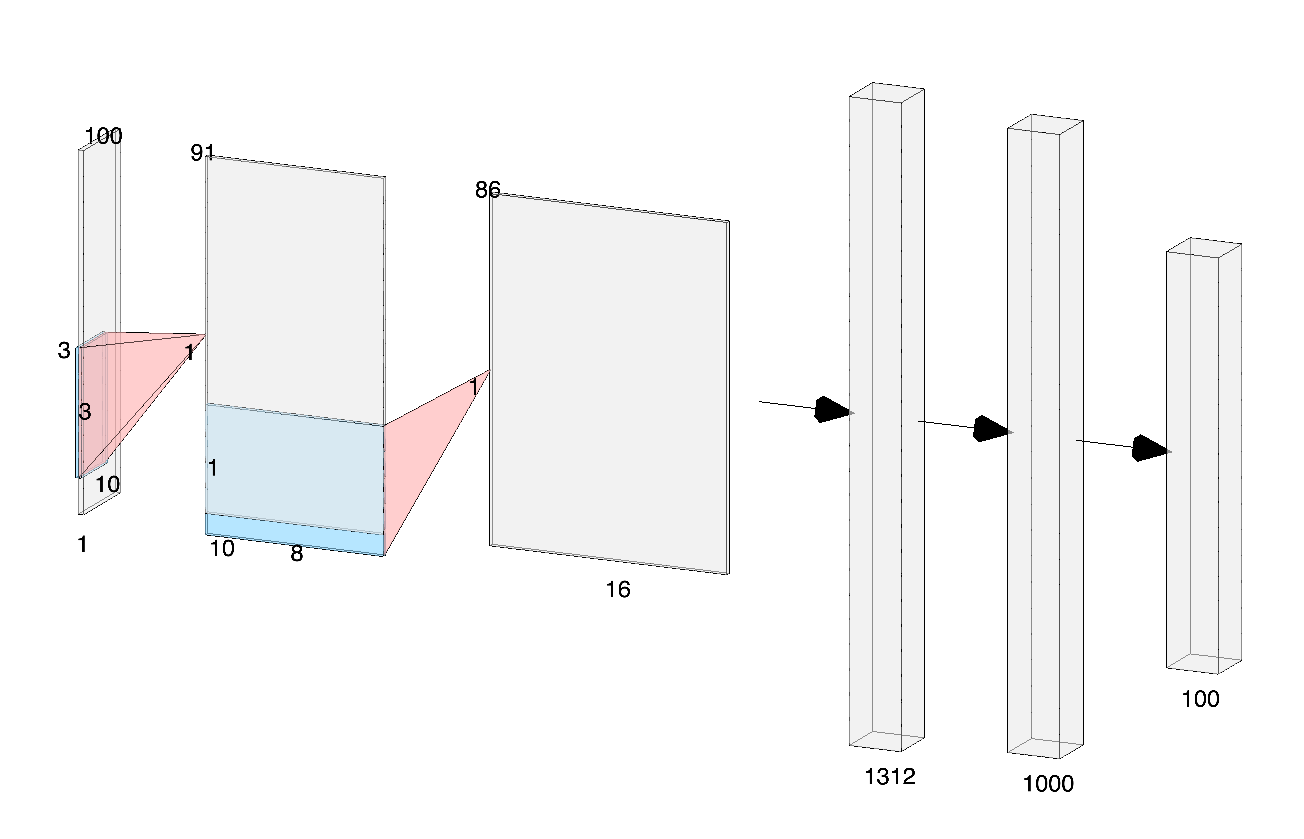
\includegraphics[width=0.38\textheight]{NN.png}
	\caption{CNN structure}
	\label{fig:nn_design}
\end{figure}


With the data being processed in the second approach, convolutional neural networks were implemented. As shown in figure \ref{fig:nn_design}, the model consists of two convolutional layers and fully connected layers as well. The input layer dimension is (100,3,1) where 100 refers to fixed cache size, 3 refers to 3-dimensional features: block number, recency, and frequency, and 1 is the number of channels. The first convolutional layer consists of 6 kernels with sizes of (10,3,1). Notably, The kernel was set as wide as the data for the model to focus on internal relations among pages in the cache. After two convolutional layers, three layers of fully connected are attached.

\section{Experiments and analysis}


\subsection{LeCar - Opt}
\begin{figure}[!ht]
	\centering 
	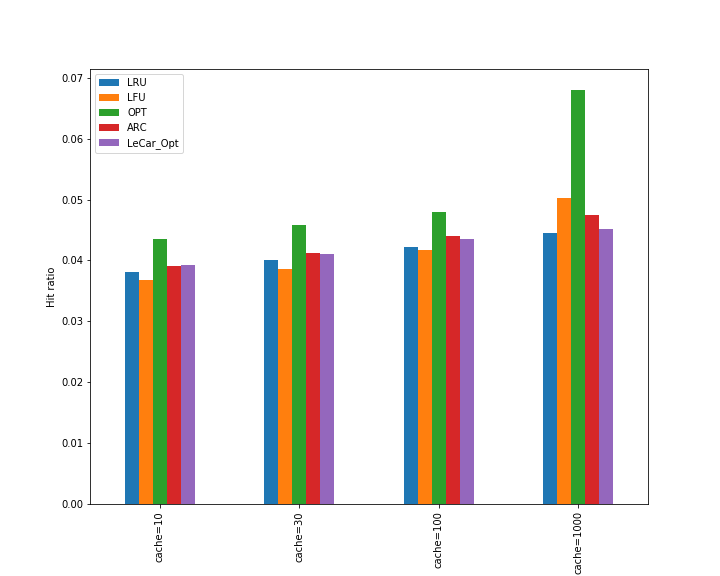
\includegraphics[width=0.38\textheight]{hitratio_bar.png}
	\caption{Hit ratio changes with different cache size on FIU workload.
}
	\label{fig:lecar_res}
\end{figure}
In figure \ref{fig:lecar_res}, LeCar\_Opt is compared with the traditional cache algorithms: LRU, LFU, ARC, and OPT. Among all these algorithms, OPT stands for the best possible hit ratio on the FIU workload. One interesting observation is when the cache size is large, LFU is the best strategy among other algorithms except for OPT, and LRU benefited the least improvement from a larger cache size. This generally shows two important characteristics of the workload dataset. First, the pages with high frequency will more likely to be accessed again in the workload. Second, the low performance of LRU with a larger cache size indicates that the workload consists of long and large sequential scan requests. Another interesting observation is that when the cache size is small, LeCar generally outperforms LRU, LFU, and ARC. When the cache size is big, LeCar\_Opt is more close to the performance of LRU. 

Figure \ref{fig:time} summarizes the efficiency of the algorithm respect to different cache size. The LeCar\_Opt is slower than ARC. However, refers to table \ref{tab:my-table}, the execution time increased linearly when the cache size grows.


\begin{figure}[!ht]
	\centering 
	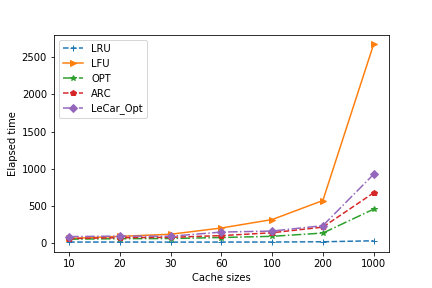
\includegraphics[width=0.38\textheight]{time.png}
	\caption{Elapsed time of running each caching algorithm with different cache size. 
}
	\label{fig:time}
\end{figure}



\begin{table}[]
\centering
\resizebox{0.5\textwidth}{!}{%
\begin{tabular}{l|l|l|l}
Cache Size & ARC Elapsed Time & LeCar\_OPT Elapsed Time & LeCar\_OPT/ARC Ratio \\ \hline
10         & 64               & 90                      & 1.40625              \\ \hline
20         & 75               & 97                      & 1.29333              \\ \hline
30         & 81               & 95                      & 1.17283              \\ \hline
60         & 104              & 151                     & 1.45192              \\ \hline
100        & 144              & 165                     & 1.14583              \\ \hline
200        & 218              & 237                     & 1.08715              \\ \hline
1000       & 677              & 926                     & 1.36779             
\end{tabular}%
}
\caption{Ratio for LeCar\_Opt elapsed time and ARC elapsed time respect to different cache size. }
\label{tab:my-table}
\end{table}
\subsection{Machine learning based approaches}

\begin{figure}[!ht]
	\centering 
	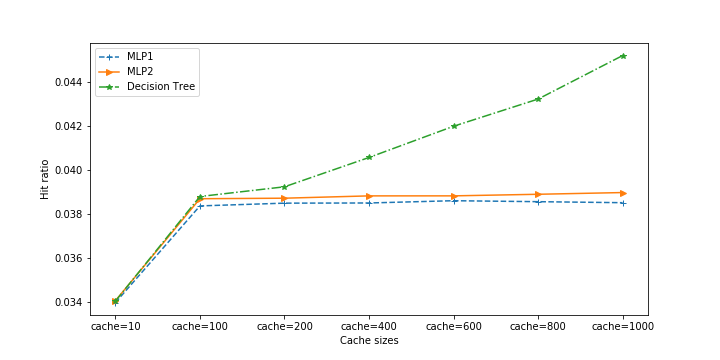
\includegraphics[width=0.38\textheight]{NN_hit.png}
	\caption{ Experiments with MLPs and Decision Tree with different cache sizes.
}
	\label{fig:nn_hit}
\end{figure}

During the experiments with ML-based approaches, hit ratio was used as the evaluation metric. We first tested with MLP with different cache sizes. As shown in figure \ref{fig:nn_hit}, a more complex network structure provides little improvement, and decision tree claimed a better performance compared to MLP. Besides, MLP did not achieve a higher hit ratio in larger cache sizes. On the contrast, the decision tree presented a steadily increased performance with different cache sizes. Then, we can summarize that a decision tree performs much better in the cache replacement scenario.

\begin{figure}[!ht]
	\centering 
	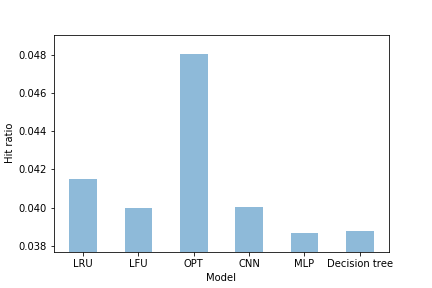
\includegraphics[width=0.38\textheight]{CNN_DNN_DT.png}
	\caption{Experiments with different ML-based models
}
	\label{fig:cnn_dnn_dt}
\end{figure}

As shown in figure \ref{fig:cnn_dnn_dt}, CNN outperforms both MLP and decision tree, and it is also slightly better than LFU. Our CNN model was constrained to learn internal relations with pages in the cache by fixing the kernel width as the same as page features, and in return, the model captured more hidden features and generated better predictions. In addition, since the designed models are all learning the OPT algorithm, it could be concluded that CNN learns the OPT pattern better than other ML-based models.  The result of outperformance is credited to the Kernels\cite{schmidhuber2015deep} design in CNN, which captures the relationships between the inputs.  


\section{Conclusion and future work}
%-------------------------------------------------------------------------------

%-------------------------------------------------------------------------------

In this project, various traditional or ML-based cache replacement algorithms have been implemented for in-depth investigation. After learning and evaluating the algorithms, one traditional algorithm, LeCar\_Opt, was proposed,  and three ML-based models were trained for the aim of improving the hit ratio on FIU workload. 

The team believes that LeCar\_Opt is a promising researching direction on policy switching based algorithms. The experiments result shows that LeCar\_Opt achieves excellent hit ratio when the cache size is small, and it is competitive with ARC when the cache size is large. However, there is still room for improvement. The current LeCar\_Opt is more sensitive to LRU pattern than LFU pattern. Therefore, it may be a better pattern the algorithm can set up in order to go against long sequential read data. 

ML-based models were also implemented for the analysis of cache replacement algorithms. Based on the different features of the models, MLP, CNN and Decision tree were explored and tuned with different hyperparameters. With enough amount of training and high complexity model,  it comes to the conclusion that ML-based algorithms are able to learn the OPT patterns on the training dataset. 












\bibliographystyle{plain}
\bibliography{report.bib}

\end{document}